\documentclass[12pt,a4paper]{article}
% \usepackage{ctex}
\usepackage{amsmath,amscd,amsbsy,amssymb,latexsym,url,bm,amsthm}
\usepackage{epsfig,graphicx,subfigure}
\usepackage{enumitem,balance}
\usepackage{wrapfig}
\usepackage{mathrsfs,euscript}
\usepackage[usenames]{xcolor}
\usepackage{hyperref}
\usepackage[vlined,ruled,linesnumbered]{algorithm2e}
\usepackage{array}
\hypersetup{colorlinks=true,linkcolor=black}

\newtheorem{theorem}{Theorem}
\newtheorem{lemma}[theorem]{Lemma}
\newtheorem{proposition}[theorem]{Proposition}
\newtheorem{corollary}[theorem]{Corollary}
\newtheorem{exercise}{Exercise}
\newtheorem*{solution}{Solution}
\newtheorem{definition}{Definition}
\theoremstyle{definition}

\renewcommand{\thefootnote}{\fnsymbol{footnote}}

\newcommand{\postscript}[2]
 {\setlength{\epsfxsize}{#2\hsize}
  \centerline{\epsfbox{#1}}}

\renewcommand{\baselinestretch}{1.0}

\setlength{\oddsidemargin}{-0.365in}
\setlength{\evensidemargin}{-0.365in}
\setlength{\topmargin}{-0.3in}
\setlength{\headheight}{0in}
\setlength{\headsep}{0in}
\setlength{\textheight}{10.1in}
\setlength{\textwidth}{7in}
\makeatletter \renewenvironment{proof}[1][Proof] {\par\pushQED{\qed}\normalfont\topsep6\p@\@plus6\p@\relax\trivlist\item[\hskip\labelsep\bfseries#1\@addpunct{.}]\ignorespaces}{\popQED\endtrivlist\@endpefalse} \makeatother
\makeatletter
\renewenvironment{solution}[1][Solution] {\par\pushQED{\qed}\normalfont\topsep6\p@\@plus6\p@\relax\trivlist\item[\hskip\labelsep\bfseries#1\@addpunct{.}]\ignorespaces}{\popQED\endtrivlist\@endpefalse} \makeatother

\begin{document}
\noindent

%========================================================================
\noindent\framebox[\linewidth]{\shortstack[c]{
\Large{\textbf{Lab08-Graph Exploration}}\vspace{1mm}\\
CS214-Algorithm and Complexity, Xiaofeng Gao \& Lei Wang, Spring 2021.}}
\begin{center}
\footnotesize{\color{red}$*$ If there is any problem, please contact TA Yihao Xie. }

\footnotesize{\color{blue}$*$ Name: Wendi Chen  \quad Student ID: 519021910071 \quad Email: chenwendi-andy@sjtu.edu.cn}
\end{center}

\begin{enumerate}

	\item Given a graph $G = (V, E)$. Prove the following propositions.
	
	\begin{enumerate}
		\item Let $e$ be a maximum-weight edge on some cycle of connected graph $G=(V,E)$.
        Then there is a minimum spanning tree of $G$ that does not include $e$. Moreover, there is no minimum spanning tree of $G$ that includes $e$ if $e$ is the unique maximum-weight edge on the cycle. 
		\item Let $T$ and $T'$ are two different minimum spanning trees of $G$. Then $T'$ can be obtained from $T$ by repeatly substitute one edge in $T\backslash T'$ by one edge in $T'\backslash T$ and meanwhile the result after each subsitution is still a minimum spanning tree.
	\end{enumerate}
	
	\begin{solution}
	~
	\begin{enumerate}
	    \item 
	    Set $m$ as an MST of $G$. If $e$ is not contained in $m$, then we have proved the conclusion. Otherwise, we can remove $e$ from $m$ and $m$ will be split into two small trees $m_1$ and $m_2$. Because $e$ is on some cycle of $G$, the cycle must connects $m_1$ and $m_2$. Thus, there exists another edge $e^{'}$ that connect $m_1$ and $m_2$, which constructs a MST that does not include $e$ (Figure \ref{Fig-MST}). Moreover, if $e$ is the unique maximum-weight edge on the cycle, then $|e^{'}|<|e|$, which means that $m$ can not be a MST. Therefore, there is no minimum spanning tree of $G$ that includes $e$. 
	    
	    \begin{figure}[htbp]
            \centering 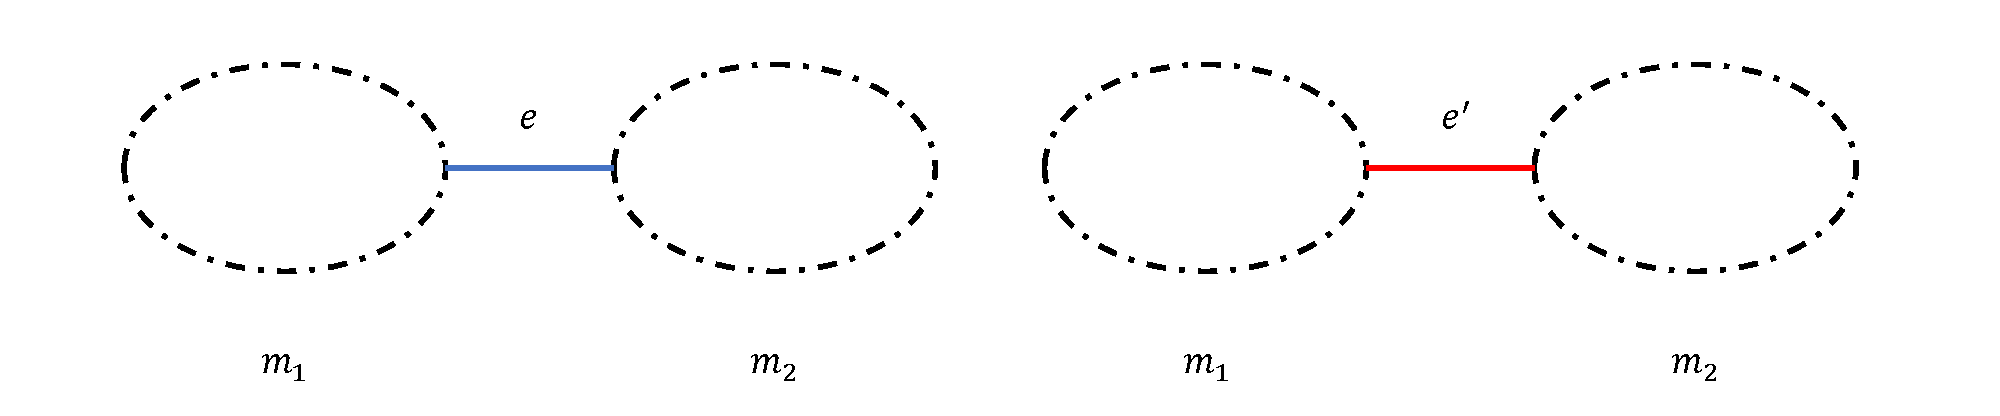
\includegraphics[width=0.8\textwidth]{Fig-MST.pdf}
            \caption{How to Find an Edge for Substitution}\label{Fig-MST}
        \end{figure}
        
        \item
        What we need to consider is the edges on some cycle of $G$ which are contained in $T^{'}$ but not in $T(T_1)$. We denote them by $e_1,e_2,\dots,e_n$. Then, let us prove by induction.\\
        We start with $i=1$. In fact, $T_1$ is a MST.\\
        We assume $T_i(i\ge 1)$ is a MST. For $e_i$, we add them to $T_i$ and $T_i$ becomes a graph $T_i^{'}$. Then, $e_i$ will construct a circle in $T_i^{'}$. Because $T_i$ is a MST, for every $e_j \neq e_i$ on the circle, we have $|e_j|\le|e_i|$. According to problem (a), there must exist $e_k\neq e_i$ so that $|e_k|=|e_i|$. Then, we'll prove that there must exist $e_q \in T_i\backslash T^{'}$ satisfying this condition. If all the edges on the circle have the same weight, it's trivial. Otherwise, if all $e_k\neq e_i$ with $|e_k| = |e_i|$ on the circle is in $T^{'}$, then we can replace one $e_k$ in $T^{'} $ with an edge with less weight, which contradicts the fact that $T^{'}$ is a MST. Thus, we can remove $e_q \in T_i\backslash T^{'}$ from $T_i^{'}$ and get $T_{i+1}$, which is also a MST.\\
        By doing this recursively, we'll finally get $T^{'}$, and $T_1(T),T_2,\dots,T_{n+1}(T^{'})$ are all MSTs.
        
        
        \begin{figure}[htbp]
            \centering 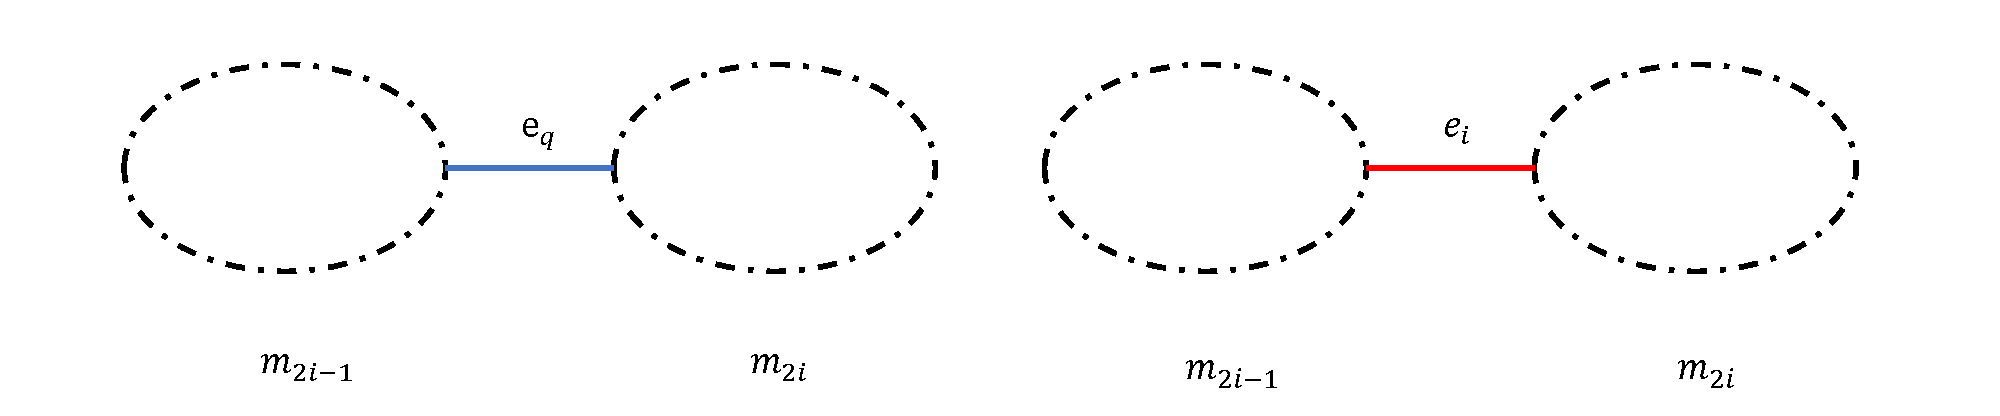
\includegraphics[width=0.8\textwidth]{Fig-substitution.pdf}
            \caption{How to Transform One MST to Another}\label{Fig-substitution}
        \end{figure}
        
	\end{enumerate}
	\end{solution}
% 	\newpage
    \item Let $G=(V,E)$ be a connected, undirected graph. Give an $O(|V|+|E|)$-time algorithm
    to compute a path in $G$ that traverses each edge in $E$ exactly once in each direction. Describe how you can find your way out of a maze if you are given a large supply of pennies.
    
    \begin{solution}
    ~\\
    \begin{minipage}[t]{0.8\textwidth}
        \begin{algorithm}[H]
        \KwIn{$G=(V,E)$ is a connected, undirected graph;$v\in V$}
        \KwOut{Sequence (not a set) $P$ which represents the path}
            		
        \BlankLine
        \caption{Traverse($G,v$)}
        \label{traverse}
        $f\leftarrow NULL$\;
        $visited(v)=true$\;
        \For{$e = edge(v,u)\in E$ }{
            \If{$count(e) = 0$ }{
                $P\leftarrow P\cup\{(v,u)\}$\;
                $count(e)\leftarrow count(e)+1$\;
                \If{$visited(u) = false$}{
                    Traverse($G,u$)\;
                }
                \Else{
                $count(e)\leftarrow count(e)+1$\;
                $P\leftarrow P\cup\{(u,v)\}$\;
                }
            }
            \ElseIf{$count(e) = 1$ }{
                $f \leftarrow e$\;
            }
        }
        \If{$f$ is not $NULL$}{
            $count(f)\leftarrow count(f)+1$\;
            $P\leftarrow P\cup\{f^{-1} = (u,v)\}$\;
        }
        \end{algorithm}
    \end{minipage}
    
    In this algorithm, every edge will be examined exactly twice and every vertex will be marked. Thus, the time complexity is $O(|V|+|E|)$.\\
    When we try to find a way out of a maze, we can put some pennies on each edge to represent $count(e)$ and then we can traverses each edge in the maze exactly once in each direction to find the route. 
    
    
    \end{solution}

    \item Consider the maze shown in Figure \ref{Fig-Maze}. The black blocks in the figure are blocks that can not be passed through. Suppose the block are explored in the order of right, down, left and up. That is, to go to the next block from $(X,Y)$, we always explore $(X,Y+1)$ first, and then $(X+1,Y)$,$(X,Y-1)$ and$(X-1,Y)$ at last. Answer the following subquestions:
    \begin{enumerate}
        \item Give the sequence of the blocks explored by using DFS to find a path from the "start" to the "finish".
        \item Give the sequence of the blocks explored by using BFS to find the \underline{shortest} path from the "start" to the "finish".
        \item Consider a maze with a larger size. Discuss which of BFS and DFS will be used to find one path and which will be used to find the shortest path from the start block to the finish block.
    \end{enumerate}
    
    \begin{figure}[!htbp]
	\centering
	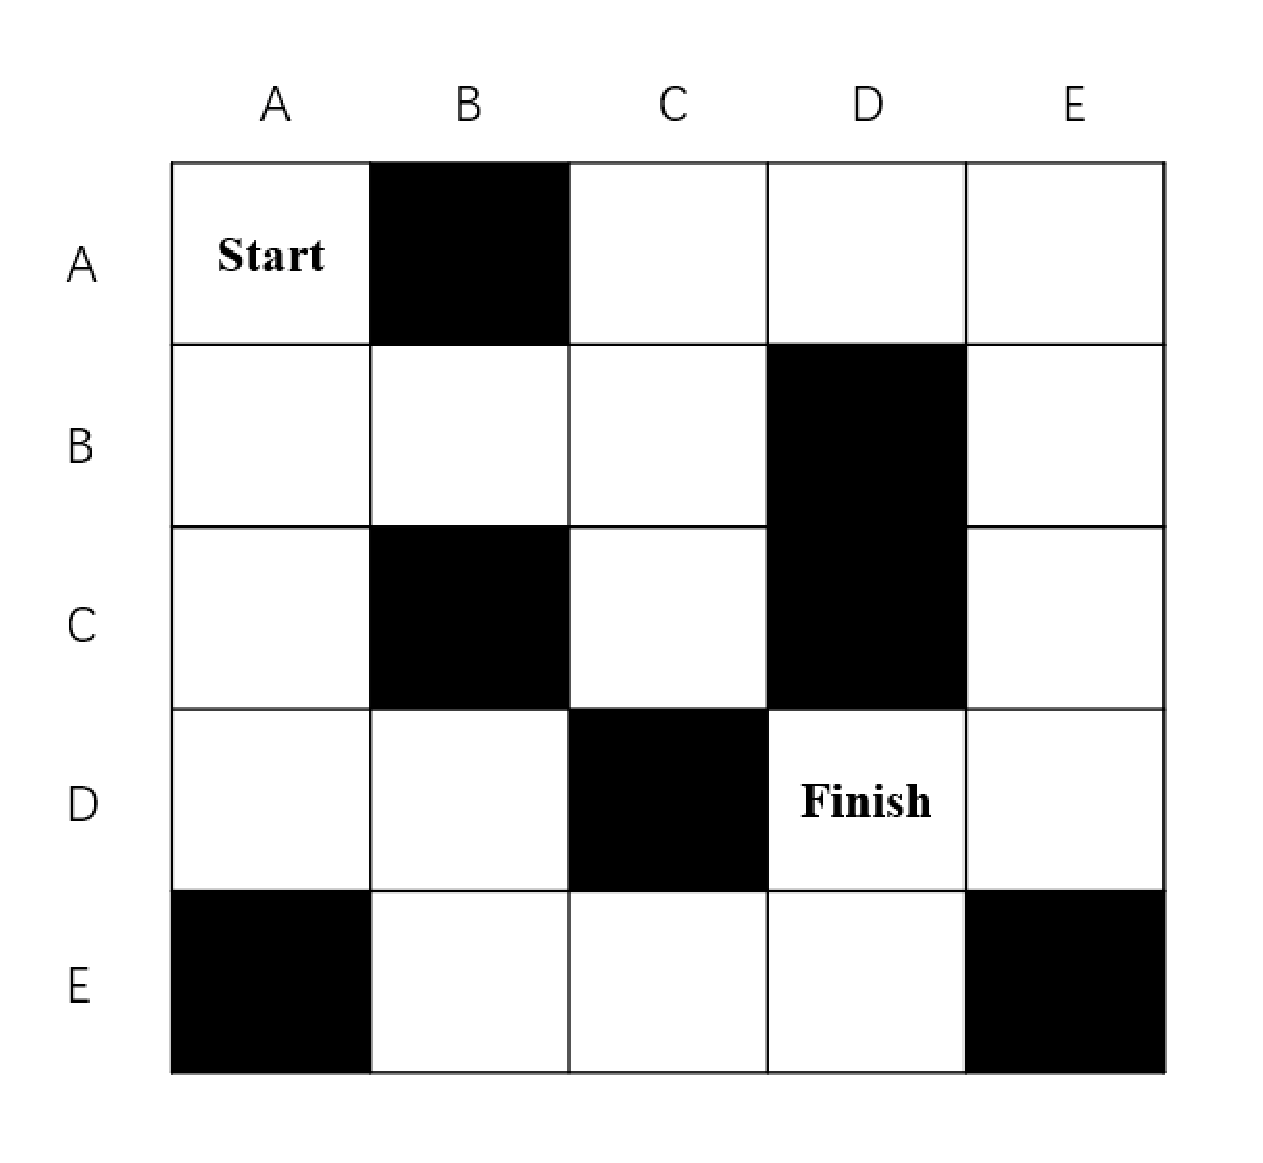
\includegraphics[width=0.5\textwidth]{Fig-Maze.pdf}
	\caption{An example of making room for one new element in the set of arrays.}
	\label{Fig-Maze}
	\end{figure}
	
	\begin{solution}
	~
	\begin{enumerate}
	    \item 
	    The sequence is $(A,A)$,$(B,A)$,$(B,B)$,$(B,C)$,$(C,C)$,$(B,C)$,$(A,C)$,$(A,D)$,$(A,E)$,$(B,E)$,\\$(C,E)$,$(D,E)$,$(D,D)$.
	    \item
	    The sequence is $(A,A)$,$(B,A)$,$(B,B)$,$(C,A)$,$(B,C)$,$(D,A)$,$(C,C)$,$(A,C)$,$(D,B)$,$(A,D)$,\\$(E,B)$,$(A,E)$,$(E,C)$,$(B,E)$,$(E,D)$,$(C,E)$,$(D,D)$.
	    \item
	    If we just want to find one path, we had better use DFS. The reason is that in DFS, we'll explore the block that far from the start block first and we try every route one by one instead of doing this parallelly. Thus, we can explore fewer blocks to get the path.\\
	    If we want to find the shortest path, we had better use BFS. The reason is that in BFS, every route we try parallelly has the same number of blocks. Then, the route arrives at the finish block first is the shortest path. If we use DFS instead, we may have to find every possible path one by one and do a comparison, which costs far more than BFS.
	\end{enumerate}
	\end{solution}
	
	\item Given a directed graph $G$, whose vertices and edges information are introduced in data file "SCC.in". Please find its number of Strongly Connected Components with respect to the following subquestions.
    
    \begin{enumerate}
    	\item Read the code and explanations of the provided C/C++ source code "SCC.cpp", and try to complete this implementation.
    	\item Visualize the above selected Strongly Connected Components for this graph $G$. Use the $Gephi$ or other software you preferred to draw the graph. {\color{blue}(If you feel that the data provided in ``SCC.in'' is not beautiful, you can also generate your own data with more vertices and edges than $G$ and draw an additional graph. Notice that results of your visualization will be taken into the consideration of Best Lab.)}
    \end{enumerate}	
    
    \begin{solution}
    ~
    \begin{enumerate}
        \item
        I use \emph{Tarjan Algorithm} to find the number of strongly connected components. Please refer to \emph{SCC.cpp} for details.
        \item
        First, we dye the vertexes in different strongly connected components with different colors and visualize the graph (Figure \ref{Fig-graph}). 
        
        \begin{figure}[!htbp]
    	\centering
    	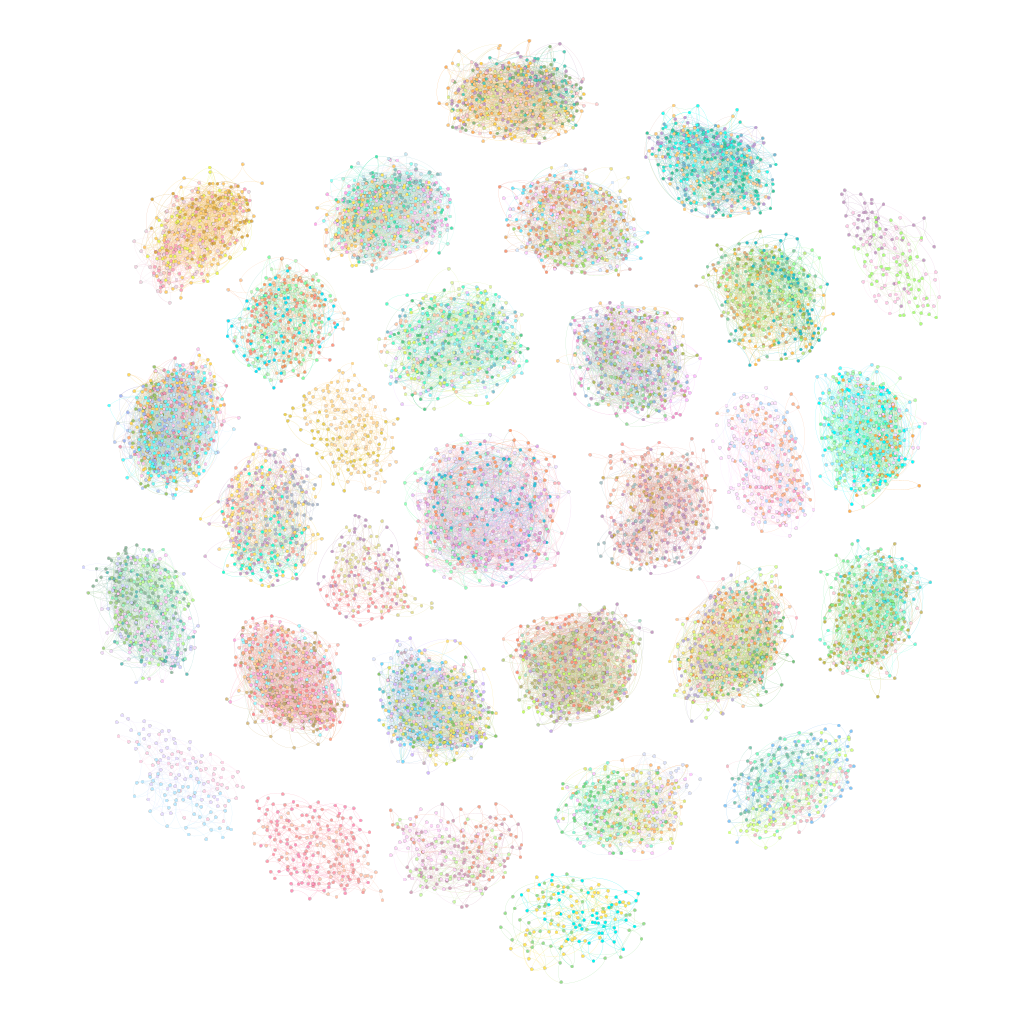
\includegraphics[width=0.5\textwidth]{Fig-graph.png}
    	\caption{Visualize the Graph with Gephi}
    	\label{Fig-graph}
    	\end{figure}
    	
        Then, I merge all the vertexes in one strongly connected components into a ``super node'' whose size implies the number of vertexes it contains. The result is much more beautiful (Figure \ref{Fig-SCC}). From the result, we can find there are 20 weakly connected components and 202 strongly connected components.
        \begin{figure}[!htbp]
    	\centering
    	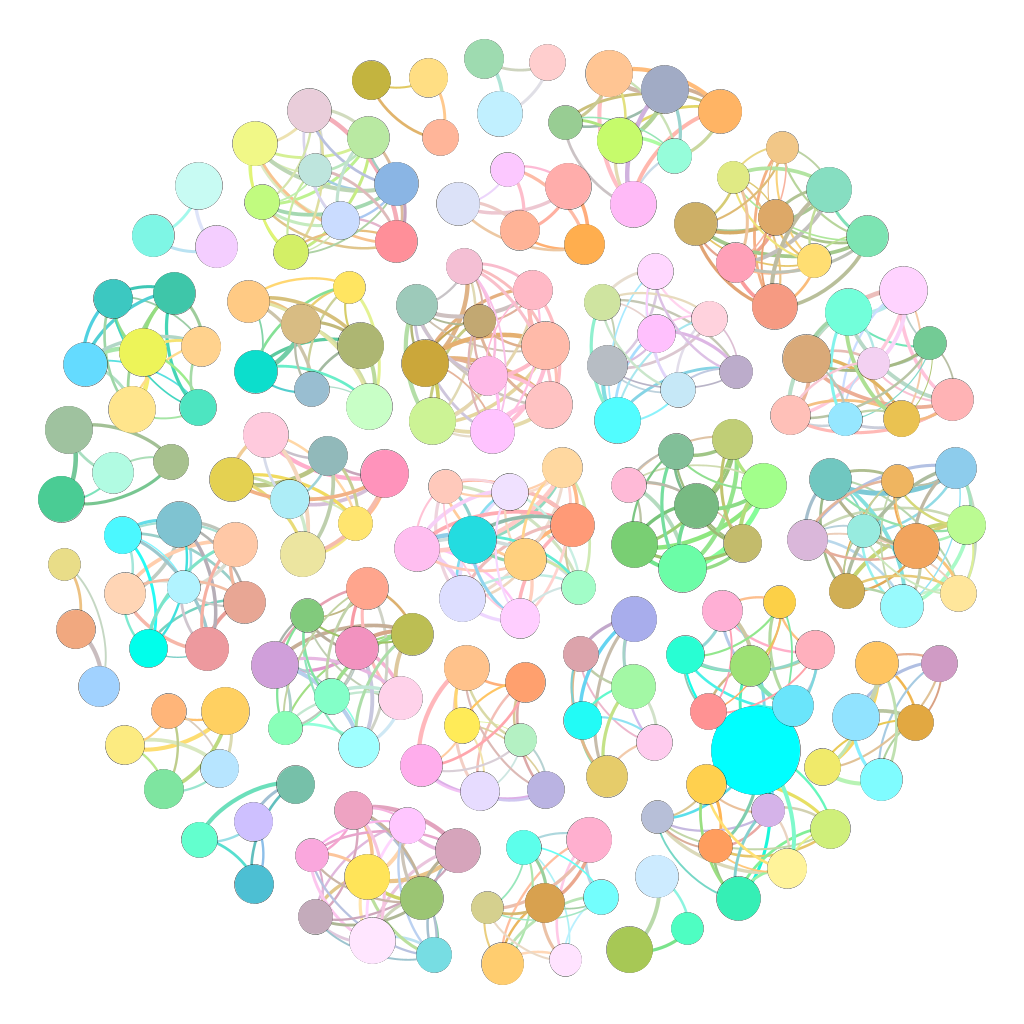
\includegraphics[width=0.5\textwidth]{Fig-SCC.png}
    	\caption{Visualize SCC with Gephi}
    	\label{Fig-SCC}
    	\end{figure}
    	\newpage
    \end{enumerate}
    \end{solution}
    
\end{enumerate}



\textbf{Remark:} Please include your .pdf, .tex, .cpp files for uploading with standard file names.
\newpage


%========================================================================
\end{document}